% !Mode:: "TeX:UTF-8" 






\BiSection{3.21}{Figures}

\fancyhead[R]{本题3.21由QC.Z完成}

假设所有MOSFET都在饱和区,计算图3.84中每个电路的小信号电压增益($\lambda  \neq 0, \gamma =0$)。

		\begin{figure}[H] %H为当前位置,!htb为忽略美学标准,htbp为浮动图形
	\begin{minipage}{\linewidth}
		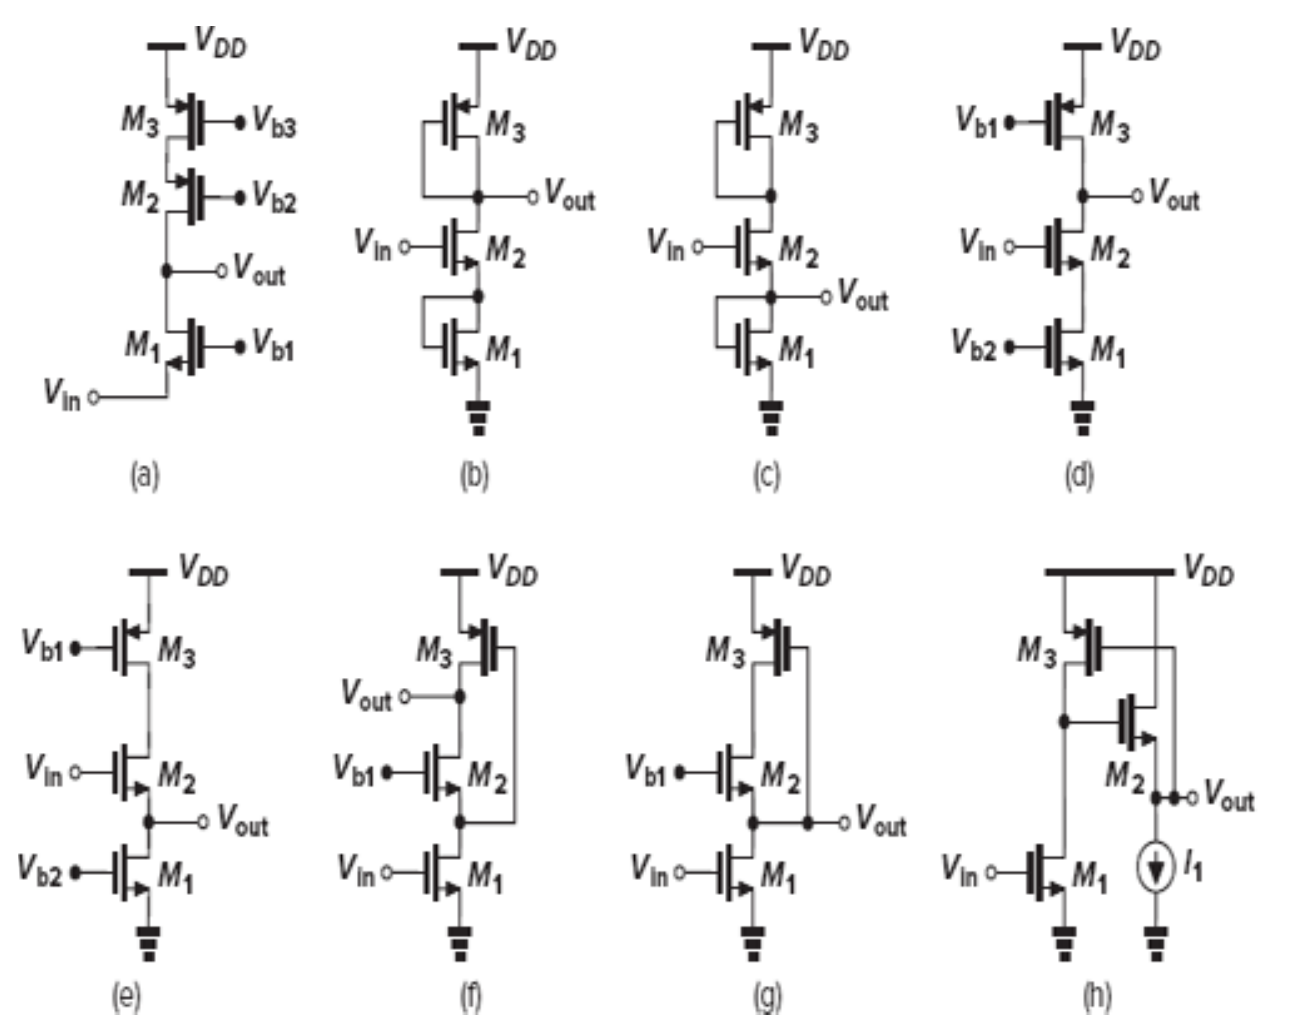
\includegraphics[width=1\linewidth]{3.21-t}
	\end{minipage}
	\caption*{图3.84} %最终文档中希望显示的图片标题
\end{figure}

解:

\scalebox{3}{(a)}

(a)重画于图1

		\begin{figure}[H] %H为当前位置,!htb为忽略美学标准,htbp为浮动图形
	\begin{minipage}{\linewidth}
		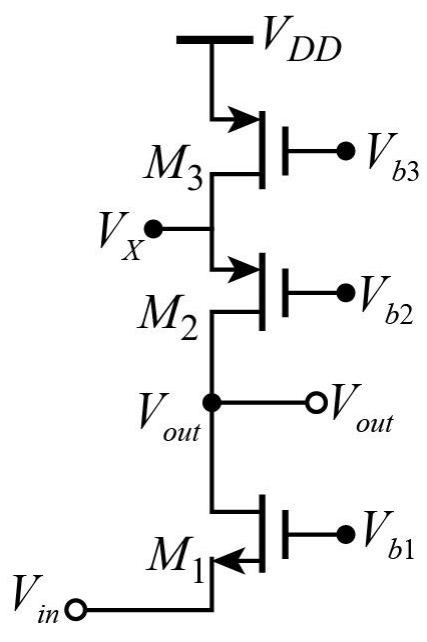
\includegraphics[width=1\linewidth]{3.21-1}
	\end{minipage}
	\caption*{图1} %最终文档中希望显示的图片标题
\end{figure}

在$V_X$点用基尔霍夫电流定律Kirchhoff’s Current Law(KCL),有$g_{m2}V_X+\frac{V_X-V_{out}}{r_{o2}}+\frac{V_X}{r_{o3}}=0$\ding{172}\textcolor{blue}{($V_{DD},V_{b1},V_{b2},V_{b3}$全部交流接地,$V_{SG2}=V_X$,$\frac{V_X}{\frac{1}{g_{m2}}}$是电流,$V_{SG1}=0$)}

$\frac{V_{out}-V_{in}}{r_{o1}}-g_{m1}V_{in}+\frac{V_X}{r_{o3}}=0$\ding{173}

化简\ding{172}

		\begin{figure}[H] %H为当前位置,!htb为忽略美学标准,htbp为浮动图形
	\begin{minipage}{\linewidth}
		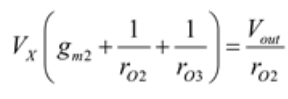
\includegraphics{3.21-2}
	\end{minipage}
\end{figure}

		\begin{figure}[H] %H为当前位置,!htb为忽略美学标准,htbp为浮动图形
	\begin{minipage}{\linewidth}
		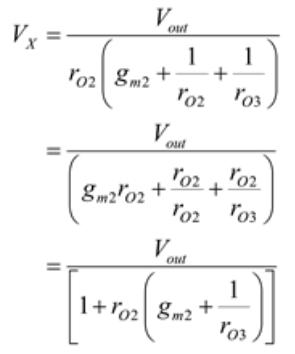
\includegraphics{3.21-3}
	\end{minipage}
\end{figure}

化简\ding{173}

		\begin{figure}[H] %H为当前位置,!htb为忽略美学标准,htbp为浮动图形
	\begin{minipage}{\linewidth}
		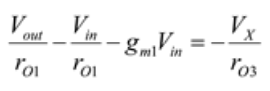
\includegraphics{3.21-4}
	\end{minipage}
\end{figure}

把上面得到的$V_X$代入得

		\begin{figure}[H] %H为当前位置,!htb为忽略美学标准,htbp为浮动图形
	\begin{minipage}{\linewidth}
		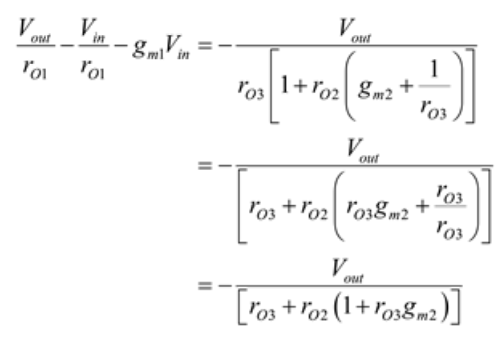
\includegraphics{3.21-5}
	\end{minipage}
\end{figure}

		\begin{figure}[H] %H为当前位置,!htb为忽略美学标准,htbp为浮动图形
	\begin{minipage}{\linewidth}
		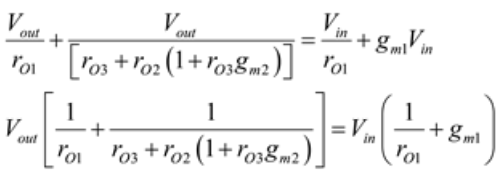
\includegraphics{3.21-6}
	\end{minipage}
\end{figure}

		\begin{figure}[H] %H为当前位置,!htb为忽略美学标准,htbp为浮动图形
	\begin{minipage}{\linewidth}
		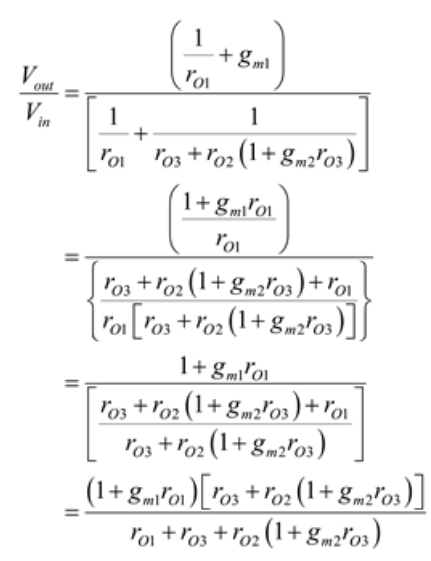
\includegraphics{3.21-7}
	\end{minipage}
\end{figure}

$A_V=\frac{V_{out}}{V_{in}}$



\begin{figure}[H] %H为当前位置,!htb为忽略美学标准,htbp为浮动图形
	\begin{minipage}{\linewidth}
		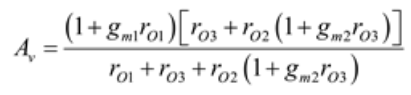
\includegraphics{3.21-8}
	\end{minipage}
\end{figure}

\scalebox{3}{(b)}

(b)重画于图2

\begin{figure}[H] %H为当前位置,!htb为忽略美学标准,htbp为浮动图形
	\begin{minipage}{\linewidth}
		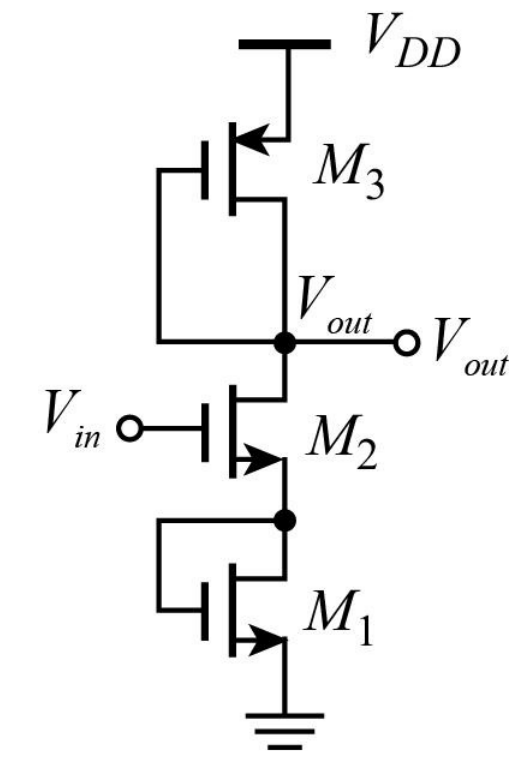
\includegraphics[width=1\linewidth]{3.21-9}
	\end{minipage}
	\caption*{图2} %最终文档中希望显示的图片标题
\end{figure}

$G_m=\frac{g_{m2}r_{o2}}{(\frac{1}{g_{m1}}||r_{o1})+r_{o2}[1+g_{m2}(\frac{1}{g_{m1}}||r_{o1})]}$

$R_{out}=(\frac{1}{g_{m3}}||r_{o3})||\{r_{o2}[1+g_{m2}(\frac{1}{g_{m1}}||r_{o1})]+(\frac{1}{g_{m1}}||r_{o1})\}$

$A_V=-G_mR_{out}$

\begin{figure}[H] %H为当前位置,!htb为忽略美学标准,htbp为浮动图形
	\begin{minipage}{\linewidth}
		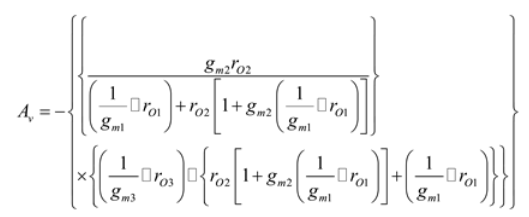
\includegraphics{3.21-10}
	\end{minipage}
\end{figure}

\begin{figure}[H] %H为当前位置,!htb为忽略美学标准,htbp为浮动图形
	\begin{minipage}{\linewidth}
		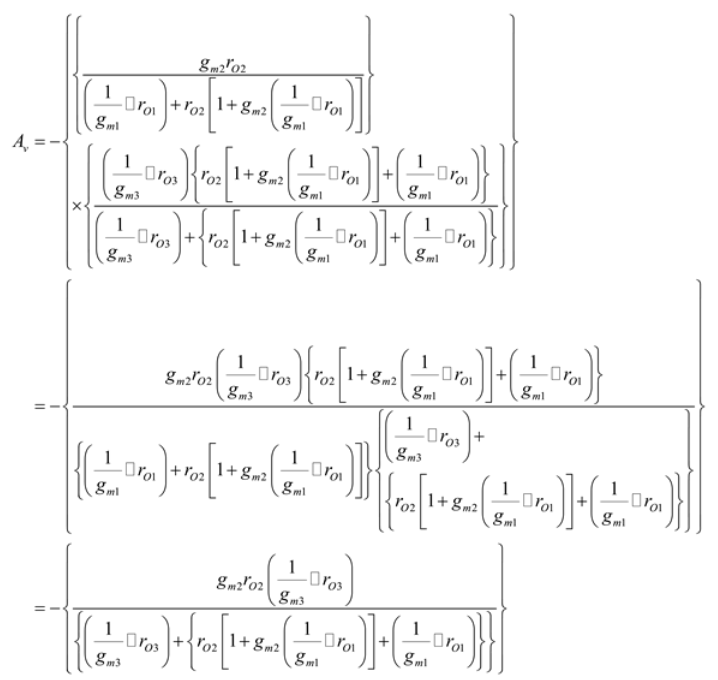
\includegraphics{3.21-11}
	\end{minipage}
\end{figure}

\scalebox{3}{(c)}

(c)重画于图3

\begin{figure}[H] %H为当前位置,!htb为忽略美学标准,htbp为浮动图形
	\begin{minipage}{\linewidth}
		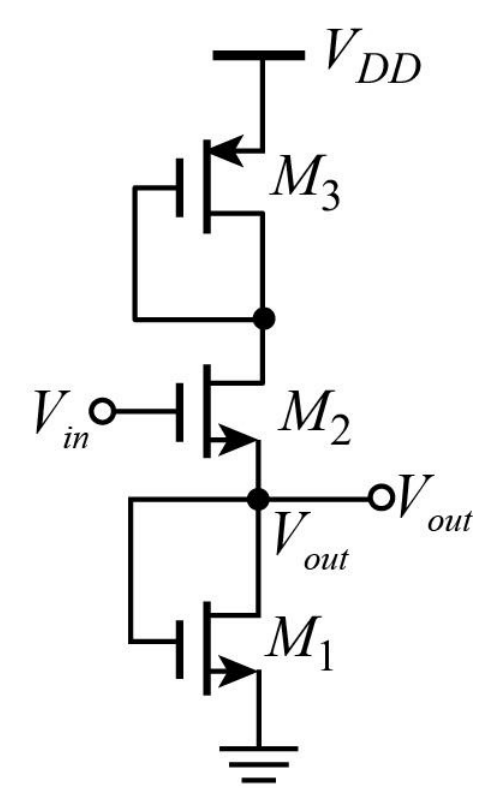
\includegraphics[width=1\linewidth]{3.21-12}
	\end{minipage}
	\caption*{图3} %最终文档中希望显示的图片标题
\end{figure}

在$V_{out}$点用基尔霍夫电流定律Kirchhoff’s Current Law(KCL),\textcolor{blue}{(注意二极管连接型器件的不同点)}有

\begin{figure}[H] %H为当前位置,!htb为忽略美学标准,htbp为浮动图形
	\begin{minipage}{\linewidth}
		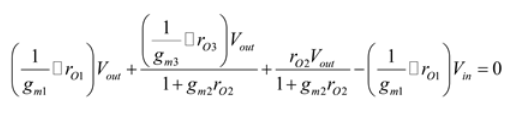
\includegraphics{3.21-13}
	\end{minipage}
\end{figure}

\begin{figure}[H] %H为当前位置,!htb为忽略美学标准,htbp为浮动图形
	\begin{minipage}{\linewidth}
		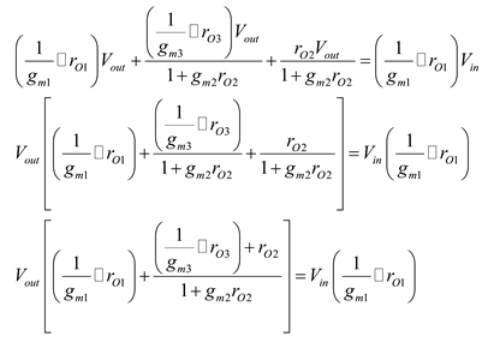
\includegraphics{3.21-14}
	\end{minipage}
\end{figure}

\begin{figure}[H] %H为当前位置,!htb为忽略美学标准,htbp为浮动图形
	\begin{minipage}{\linewidth}
		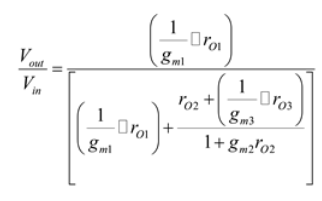
\includegraphics{3.21-15}
	\end{minipage}
\end{figure}

\begin{figure}[H] %H为当前位置,!htb为忽略美学标准,htbp为浮动图形
	\begin{minipage}{\linewidth}
		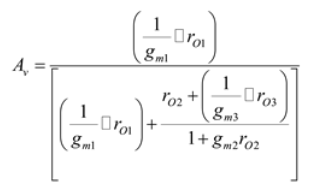
\includegraphics{3.21-16}
	\end{minipage}
\end{figure}

\scalebox{3}{(d)}

(d)重画于图4

\begin{figure}[H] %H为当前位置,!htb为忽略美学标准,htbp为浮动图形
	\begin{minipage}{\linewidth}
		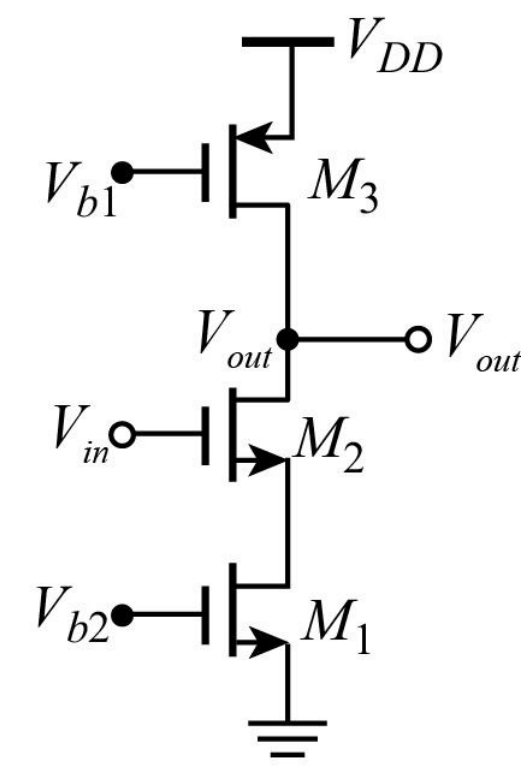
\includegraphics[width=1\linewidth]{3.21-17}
	\end{minipage}
	\caption*{图4} %最终文档中希望显示的图片标题
\end{figure}

\begin{figure}[H] %H为当前位置,!htb为忽略美学标准,htbp为浮动图形
	\begin{minipage}{\linewidth}
		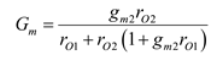
\includegraphics{3.21-18}
	\end{minipage}
\end{figure}

\begin{figure}[H] %H为当前位置,!htb为忽略美学标准,htbp为浮动图形
	\begin{minipage}{\linewidth}
		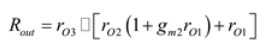
\includegraphics{3.21-19}
	\end{minipage}
\end{figure}

\begin{figure}[H] %H为当前位置,!htb为忽略美学标准,htbp为浮动图形
	\begin{minipage}{\linewidth}
		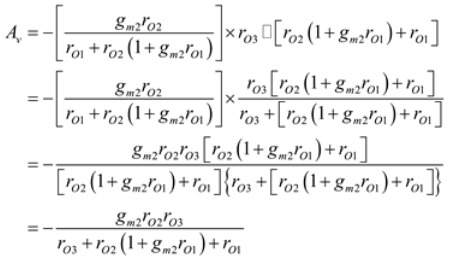
\includegraphics{3.21-20}
	\end{minipage}
\end{figure}

\scalebox{3}{(e)}

(e)重画于图5

\begin{figure}[H] %H为当前位置,!htb为忽略美学标准,htbp为浮动图形
	\begin{minipage}{\linewidth}
		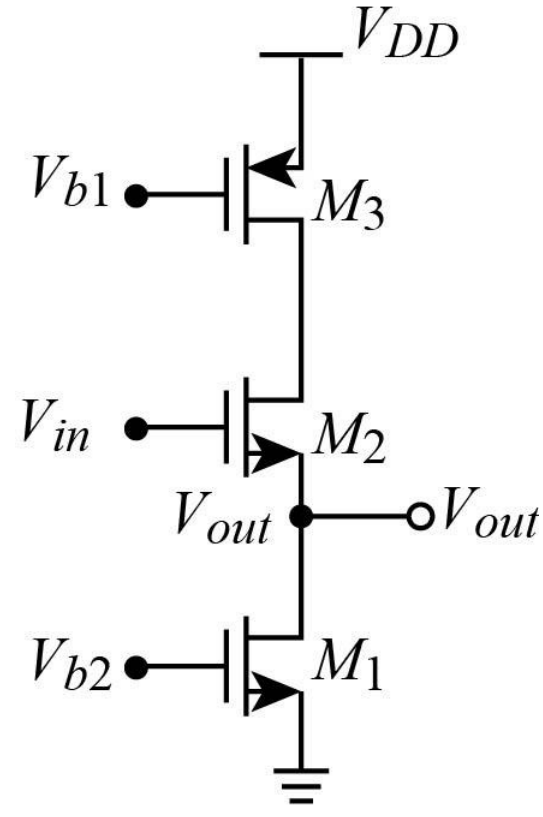
\includegraphics[width=1\linewidth]{3.21-21}
	\end{minipage}
	\caption*{图5} %最终文档中希望显示的图片标题
\end{figure}

在$V_{out}$点用基尔霍夫电流定律Kirchhoff’s Current Law(KCL),有

\begin{figure}[H] %H为当前位置,!htb为忽略美学标准,htbp为浮动图形
	\begin{minipage}{\linewidth}
		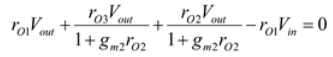
\includegraphics{3.21-22}
	\end{minipage}
\end{figure}

\begin{figure}[H] %H为当前位置,!htb为忽略美学标准,htbp为浮动图形
	\begin{minipage}{\linewidth}
		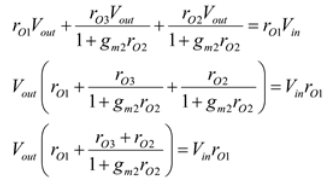
\includegraphics{3.21-23}
	\end{minipage}
\end{figure}

\begin{figure}[H] %H为当前位置,!htb为忽略美学标准,htbp为浮动图形
	\begin{minipage}{\linewidth}
		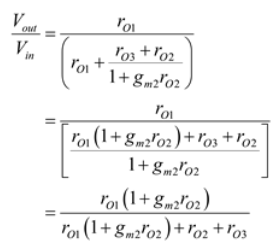
\includegraphics{3.21-24}
	\end{minipage}
\end{figure}

\begin{figure}[H] %H为当前位置,!htb为忽略美学标准,htbp为浮动图形
	\begin{minipage}{\linewidth}
		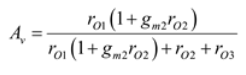
\includegraphics{3.21-25}
	\end{minipage}
\end{figure}

\scalebox{3}{(f)}

(f)重画于图6

\begin{figure}[H] %H为当前位置,!htb为忽略美学标准,htbp为浮动图形
	\begin{minipage}{\linewidth}
		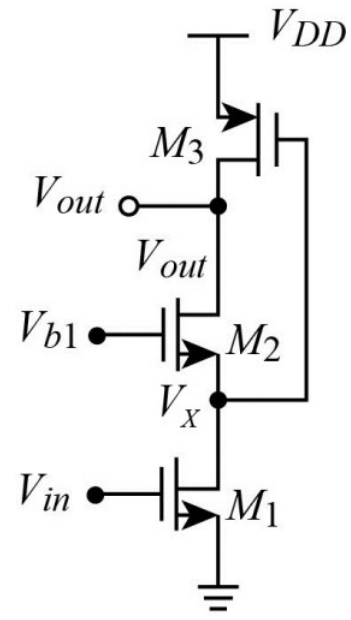
\includegraphics[width=1\linewidth]{3.21-26}
	\end{minipage}
	\caption*{图6} %最终文档中希望显示的图片标题
\end{figure}

在$V_{out}$点和$V_{out}$点用基尔霍夫电流定律Kirchhoff’s Current Law(KCL),有

\begin{figure}[H] %H为当前位置,!htb为忽略美学标准,htbp为浮动图形
	\begin{minipage}{\linewidth}
		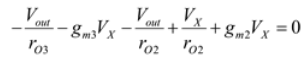
\includegraphics{3.21-27}
	\end{minipage}
\end{figure}

\begin{figure}[H] %H为当前位置,!htb为忽略美学标准,htbp为浮动图形
	\begin{minipage}{\linewidth}
		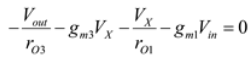
\includegraphics{3.21-28}
	\end{minipage}
\end{figure}

下面化简上面第一式

\begin{figure}[H] %H为当前位置,!htb为忽略美学标准,htbp为浮动图形
	\begin{minipage}{\linewidth}
		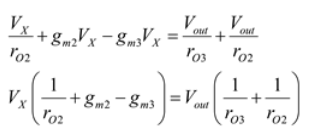
\includegraphics{3.21-29}
	\end{minipage}
\end{figure}

\begin{figure}[H] %H为当前位置,!htb为忽略美学标准,htbp为浮动图形
	\begin{minipage}{\linewidth}
		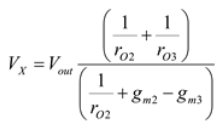
\includegraphics{3.21-30}
	\end{minipage}
\end{figure}

下面化简上面第二式

\begin{figure}[H] %H为当前位置,!htb为忽略美学标准,htbp为浮动图形
	\begin{minipage}{\linewidth}
		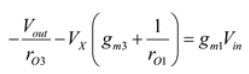
\includegraphics{3.21-31}
	\end{minipage}
\end{figure}

把上面得到的$V_X$代入得

\begin{figure}[H] %H为当前位置,!htb为忽略美学标准,htbp为浮动图形
	\begin{minipage}{\linewidth}
		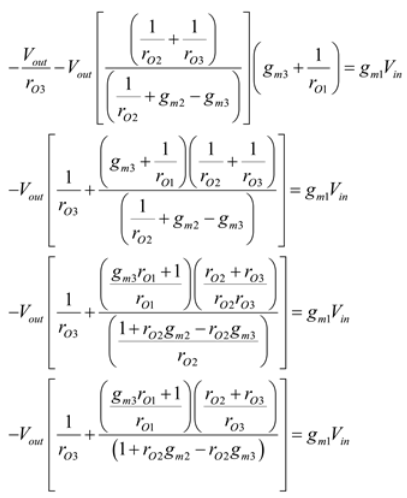
\includegraphics{3.21-32}
	\end{minipage}
\end{figure}

\begin{figure}[H] %H为当前位置,!htb为忽略美学标准,htbp为浮动图形
	\begin{minipage}{\linewidth}
		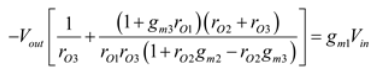
\includegraphics{3.21-33}
	\end{minipage}
\end{figure}

\begin{figure}[H] %H为当前位置,!htb为忽略美学标准,htbp为浮动图形
	\begin{minipage}{\linewidth}
		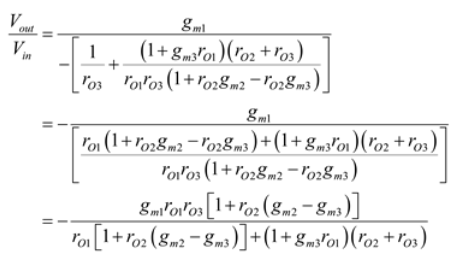
\includegraphics{3.21-34}
	\end{minipage}
\end{figure}

\begin{figure}[H] %H为当前位置,!htb为忽略美学标准,htbp为浮动图形
	\begin{minipage}{\linewidth}
		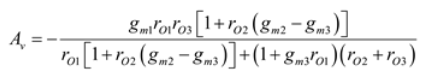
\includegraphics{3.21-35}
	\end{minipage}
\end{figure}

\scalebox{3}{(g)}

(g)重画于图7

\begin{figure}[H] %H为当前位置,!htb为忽略美学标准,htbp为浮动图形
	\begin{minipage}{\linewidth}
		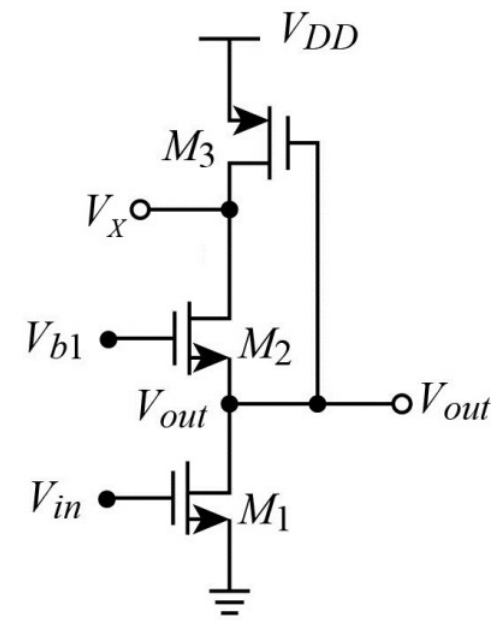
\includegraphics[width=1\linewidth]{3.21-36}
	\end{minipage}
	\caption*{图7} %最终文档中希望显示的图片标题
\end{figure}

在$V_{out}$点和$V_{out}$点用基尔霍夫电流定律Kirchhoff’s Current Law(KCL),有

\begin{figure}[H] %H为当前位置,!htb为忽略美学标准,htbp为浮动图形
	\begin{minipage}{\linewidth}
		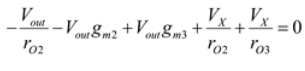
\includegraphics{3.21-37}
	\end{minipage}
\end{figure}

\begin{figure}[H] %H为当前位置,!htb为忽略美学标准,htbp为浮动图形
	\begin{minipage}{\linewidth}
		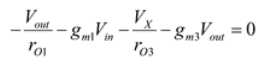
\includegraphics{3.21-38}
	\end{minipage}
\end{figure}

下面化简上面第一式

\begin{figure}[H] %H为当前位置,!htb为忽略美学标准,htbp为浮动图形
	\begin{minipage}{\linewidth}
		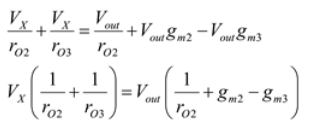
\includegraphics{3.21-39}
	\end{minipage}
\end{figure}

\begin{figure}[H] %H为当前位置,!htb为忽略美学标准,htbp为浮动图形
	\begin{minipage}{\linewidth}
		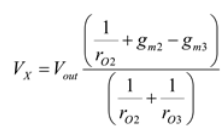
\includegraphics{3.21-40}
	\end{minipage}
\end{figure}

下面化简上面第二式

\begin{figure}[H] %H为当前位置,!htb为忽略美学标准,htbp为浮动图形
	\begin{minipage}{\linewidth}
		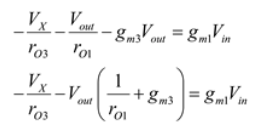
\includegraphics{3.21-41}
	\end{minipage}
\end{figure}

把上面得到的$V_X$代入得

\begin{figure}[H] %H为当前位置,!htb为忽略美学标准,htbp为浮动图形
	\begin{minipage}{\linewidth}
		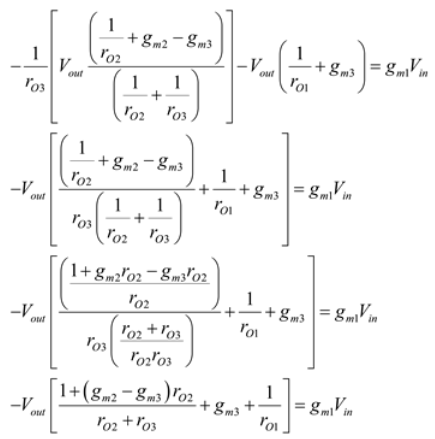
\includegraphics{3.21-42}
	\end{minipage}
\end{figure}

\begin{figure}[H] %H为当前位置,!htb为忽略美学标准,htbp为浮动图形
	\begin{minipage}{\linewidth}
		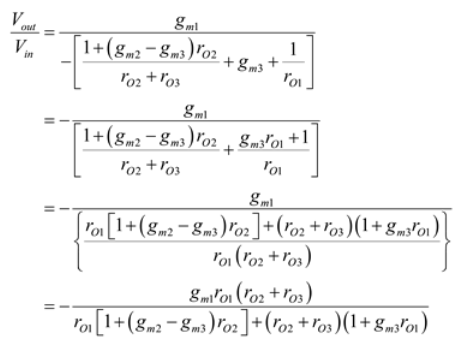
\includegraphics{3.21-43}
	\end{minipage}
\end{figure}

\begin{figure}[H] %H为当前位置,!htb为忽略美学标准,htbp为浮动图形
	\begin{minipage}{\linewidth}
		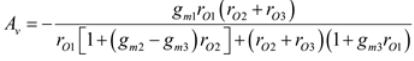
\includegraphics{3.21-44}
	\end{minipage}
\end{figure}

\scalebox{3}{(h)}

(h)重画于图8

\begin{figure}[H] %H为当前位置,!htb为忽略美学标准,htbp为浮动图形
	\begin{minipage}{\linewidth}
		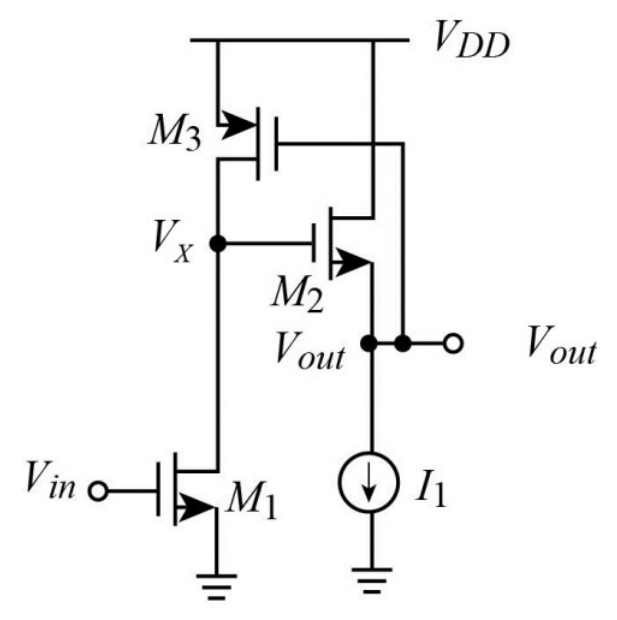
\includegraphics[width=1\linewidth]{3.21-45}
	\end{minipage}
	\caption*{图8} %最终文档中希望显示的图片标题
\end{figure}

在$V_{out}$点和$V_{out}$点用基尔霍夫电流定律Kirchhoff’s Current Law(KCL),有

\begin{figure}[H] %H为当前位置,!htb为忽略美学标准,htbp为浮动图形
	\begin{minipage}{\linewidth}
		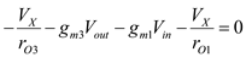
\includegraphics{3.21-46}
	\end{minipage}
\end{figure}

\begin{figure}[H] %H为当前位置,!htb为忽略美学标准,htbp为浮动图形
	\begin{minipage}{\linewidth}
		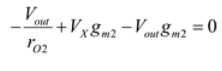
\includegraphics{3.21-47}
	\end{minipage}
\end{figure}

下面化简上面第一式

\begin{figure}[H] %H为当前位置,!htb为忽略美学标准,htbp为浮动图形
	\begin{minipage}{\linewidth}
		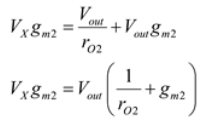
\includegraphics{3.21-48}
	\end{minipage}
\end{figure}

\begin{figure}[H] %H为当前位置,!htb为忽略美学标准,htbp为浮动图形
	\begin{minipage}{\linewidth}
		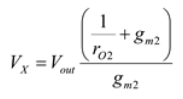
\includegraphics{3.21-49}
	\end{minipage}
\end{figure}

下面化简上面第二式

\begin{figure}[H] %H为当前位置,!htb为忽略美学标准,htbp为浮动图形
	\begin{minipage}{\linewidth}
		\includegraphics{3.21-50}
	\end{minipage}
\end{figure}

把上面得到的$V_X$代入得

\begin{figure}[H] %H为当前位置,!htb为忽略美学标准,htbp为浮动图形
	\begin{minipage}{\linewidth}
		\includegraphics{3.21-51}
	\end{minipage}
\end{figure}

\begin{figure}[H] %H为当前位置,!htb为忽略美学标准,htbp为浮动图形
	\begin{minipage}{\linewidth}
		\includegraphics{3.21-52}
	\end{minipage}
\end{figure}

\begin{figure}[H] %H为当前位置,!htb为忽略美学标准,htbp为浮动图形
	\begin{minipage}{\linewidth}
		\includegraphics{3.21-53}
	\end{minipage}
\end{figure}

